\chapter*{Annexes}
\addcontentsline{toc}{chapter}{Annexes}

\section*{Bibliothèques utilisées pour l'EDA}
\begin{figure}[H]
	\centering
	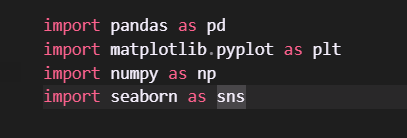
\includegraphics[width=0.7\textwidth]{../figures/importation_01.png}
\end{figure}
\noindent \textbf{Explication :} 
\texttt{pandas} pour la manipulation des données, 
\texttt{matplotlib} et \texttt{seaborn} pour la visualisation graphique, 
\texttt{numpy} pour les calculs numériques.

\section*{Chargement du dataset}
\begin{figure}[H]
	\centering
	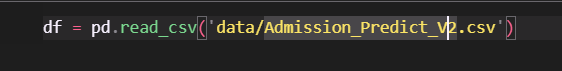
\includegraphics[width=0.7\textwidth]{../figures/load_dataset.png}
\end{figure}
\noindent \textbf{Explication :} 
La fonction \texttt{pd.read\_csv()} permet de charger le dataset afin de l’exploiter pour l’analyse et la modélisation.

\section*{Affichage des premières lignes du dataset}
\begin{figure}[H]
	\centering
	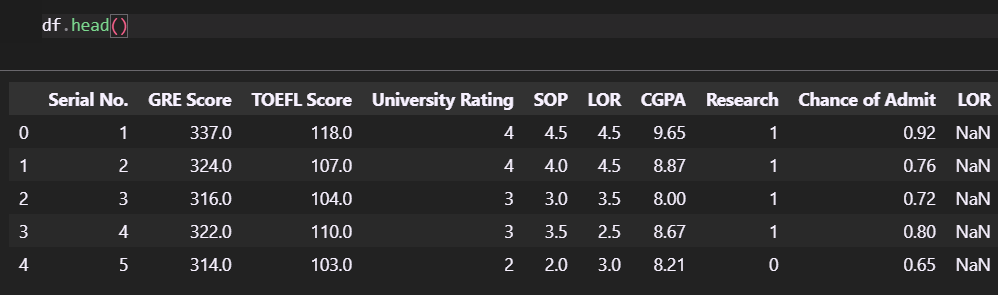
\includegraphics[width=0.9\textwidth]{../figures/head_5}
\end{figure}
\noindent \textbf{Explication :} 
La méthode \texttt{df.head()} affiche les cinq premières lignes du dataset pour un aperçu rapide de sa structure.

\section*{Aperçu du type des données}
\begin{figure}[H]
	\centering
	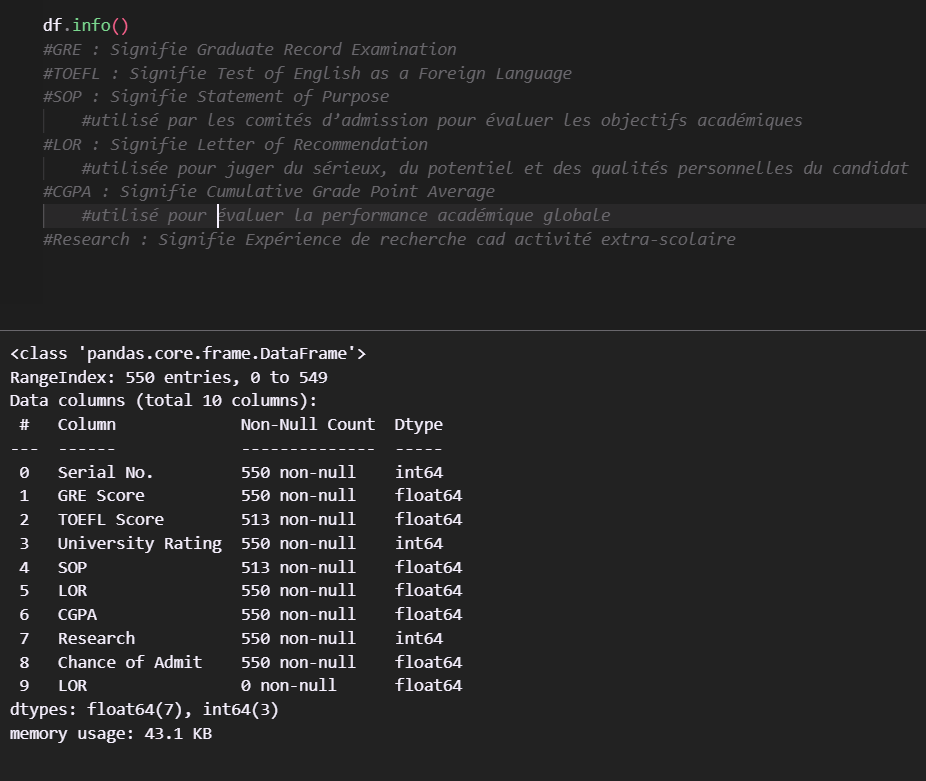
\includegraphics[width=0.9\textwidth]{../figures/info_dataset.png}
\end{figure}
\noindent \textbf{Explication :} 
\texttt{df.info()} fournit un résumé des types de données et du nombre de valeurs non nulles par colonne.

\section*{Résumé statistique du dataset}
\begin{figure}[H]
	\centering
	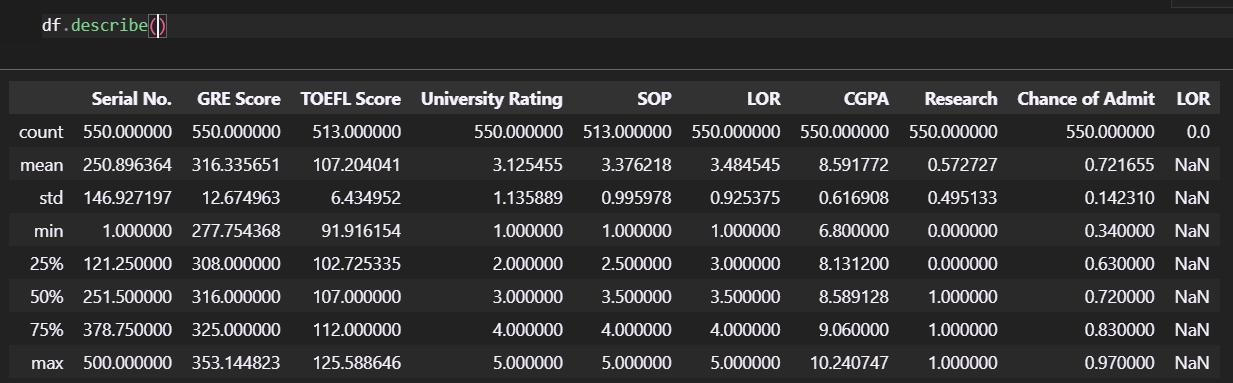
\includegraphics[width=0.9\textwidth]{../figures/describe_dataset.png}
\end{figure}
\noindent \textbf{Explication :} 
\texttt{df.describe()} calcule des statistiques descriptives : moyenne, écart-type, valeurs minimales et maximales.

\section*{Suppression des colonnes inutiles}
\begin{figure}[H]
	\centering
	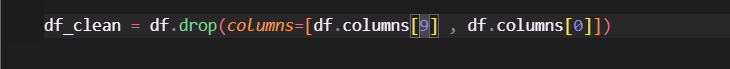
\includegraphics[width=0.9\textwidth]{../figures/remove_c.png}
\end{figure}
\noindent \textbf{Explication :} 
La colonne \texttt{Serial No.} et le doublon \texttt{LOR} ont été supprimés car non pertinents pour l’analyse.

\section*{Nettoyage des données}
\begin{figure}[H]
	\centering
	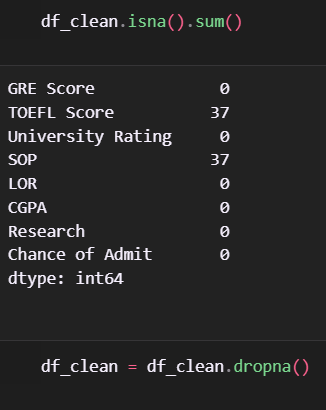
\includegraphics[width=0.9\textwidth]{../figures/cleaning_d.png}
\end{figure}
\noindent \textbf{Explication :} 
\texttt{df\_clean.isna().sum()} permet de compter les valeurs manquantes.  
Elles ont ensuite été supprimées avec \texttt{df\_clean.dropna()}.

\section*{Visualisation univariée des données}
\begin{figure}[H]
	\centering
	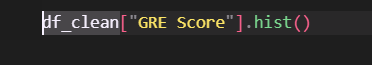
\includegraphics[width=0.9\textwidth]{../figures/v1.png}
	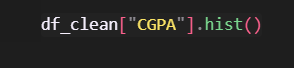
\includegraphics[width=0.9\textwidth]{../figures/v2.png}
	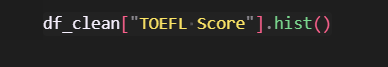
\includegraphics[width=0.9\textwidth]{../figures/v3.png}
	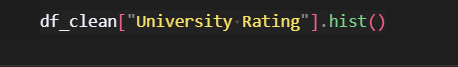
\includegraphics[width=0.9\textwidth]{../figures/v4.png}
	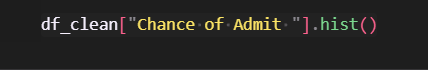
\includegraphics[width=0.9\textwidth]{../figures/v5.png}
	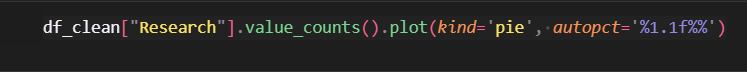
\includegraphics[width=0.9\textwidth]{../figures/v6.png}
\end{figure}
\noindent \textbf{Explication :} 
Ces codes présentent la distribution de chaque variable individuelle.

\section*{Visualisation bivariée des données}
\begin{figure}[H]
	\centering
	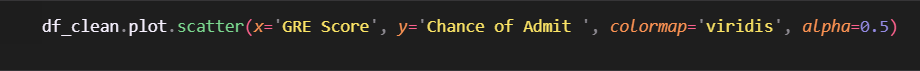
\includegraphics[width=0.9\textwidth]{../figures/b1.png}
	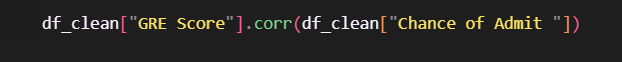
\includegraphics[width=0.9\textwidth]{../figures/b2.png}
	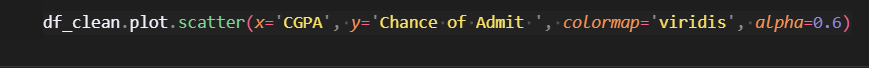
\includegraphics[width=0.9\textwidth]{../figures/b3.png}
	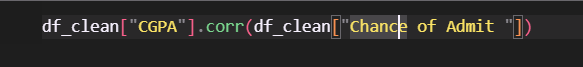
\includegraphics[width=0.9\textwidth]{../figures/b4.png}
	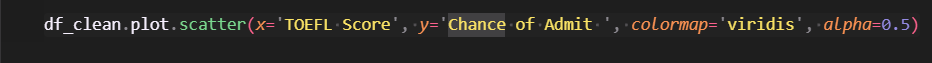
\includegraphics[width=0.9\textwidth]{../figures/b5.png}
	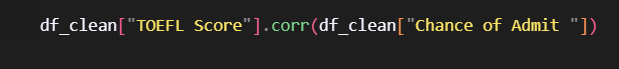
\includegraphics[width=0.9\textwidth]{../figures/b6.png}
	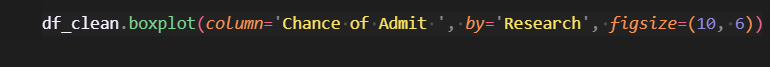
\includegraphics[width=0.9\textwidth]{../figures/b7.png}
	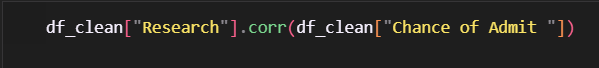
\includegraphics[width=0.9\textwidth]{../figures/b8.png}
	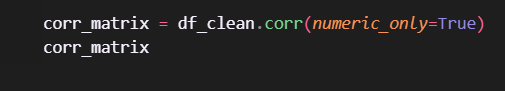
\includegraphics[width=0.9\textwidth]{../figures/b9.png}
	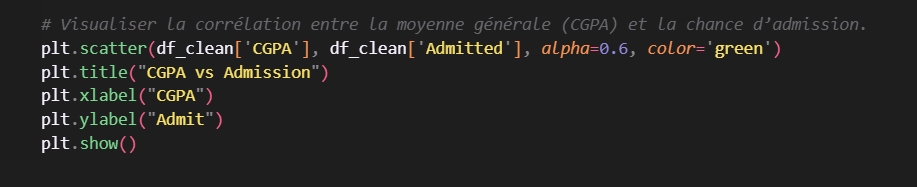
\includegraphics[width=0.9\textwidth]{../figures/b10.png}
	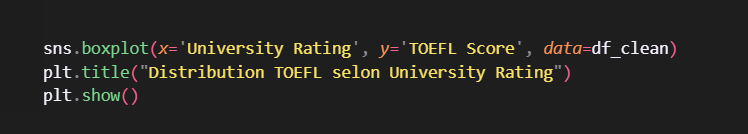
\includegraphics[width=0.9\textwidth]{../figures/b11.png}
	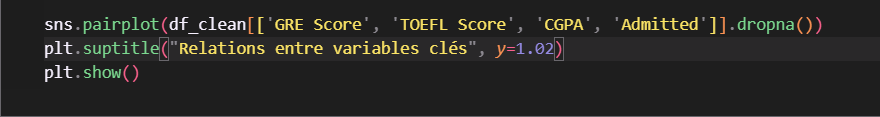
\includegraphics[width=0.9\textwidth]{../figures/b12.png}
\end{figure}
\noindent \textbf{Explication :} 
Ces codes montrent les relations entre deux variables, utiles pour détecter corrélations et tendances.

\section*{Variables utilisées pour l’entraînement du modèle (régression)}
\begin{figure}[H]
	\centering
	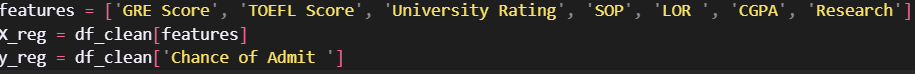
\includegraphics[width=0.9\textwidth]{../figures/regression.png}
\end{figure}

\section*{Variables utilisées pour l’entraînement du modèle (classification)}
\begin{figure}[H]
	\centering
	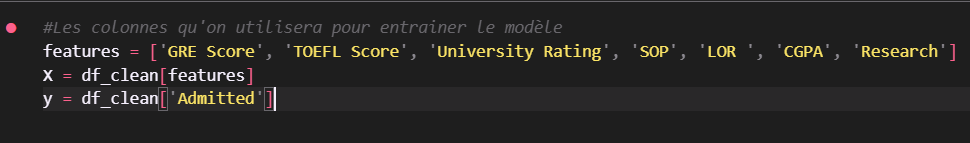
\includegraphics[width=0.9\textwidth]{../figures/v_u.png}
\end{figure}

\section*{Bibliothèques utilisées pour l’entraînement du modèle}
\begin{figure}[H]
	\centering
	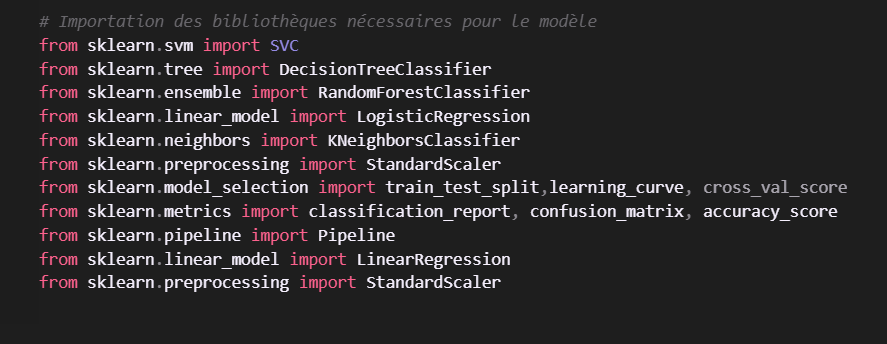
\includegraphics[width=0.9\textwidth]{../figures/b_u.png}
\end{figure}
\noindent \textbf{Imports principaux :}
\begin{itemize}
	\item \texttt{from sklearn.svm import SVC} : Support Vector Classifier.  
	\item \texttt{from sklearn.tree import DecisionTreeClassifier} : Arbre de décision.  
	\item \texttt{from sklearn.ensemble import RandomForestClassifier} : Forêt aléatoire.  
s	\item \texttt{from sklearn.linear_model import LogisticRegression, LinearRegression} : Régression logistique et linéaire.  
	\item \texttt{from sklearn.neighbors import KNeighborsClassifier} : K plus proches voisins.  
	\item \texttt{from sklearn.preprocessing import StandardScaler} : Normalisation des données.  
	\item \texttt{from sklearn.model_selection import train\_test\_split, learning\_curve, cross\_val\_score} : Division données et validation croisée.  
	\item \texttt{from sklearn.metrics import classification\_report, confusion\_matrix, accuracy\_score} : Métriques d’évaluation.  
	\item \texttt{from sklearn.pipeline import Pipeline} : Chaîne de traitement complète.  
s\end{itemize}

\section*{Exemple de code utilisé pour l’entraînement du modèle}
\begin{figure}[H]
	\centering
	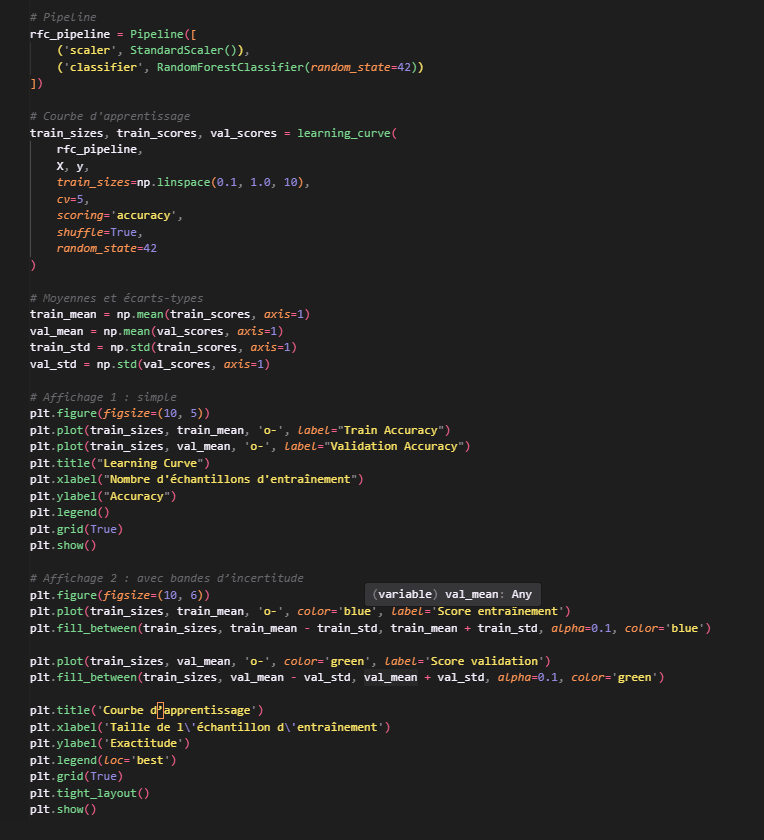
\includegraphics[width=0.9\textwidth]{../figures/E_u_t.png}
\end{figure}

\section*{Exemple de code utilisé pour tester le modèle}
\begin{figure}[H]
	\centering
	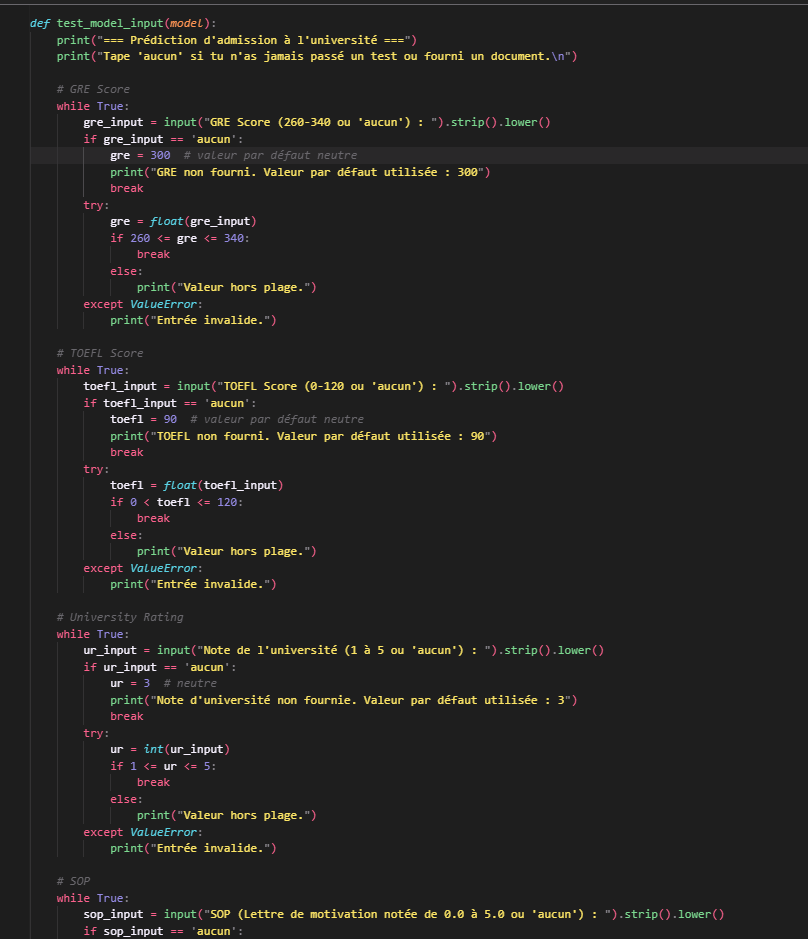
\includegraphics[width=0.9\textwidth]{../figures/t1.png}
	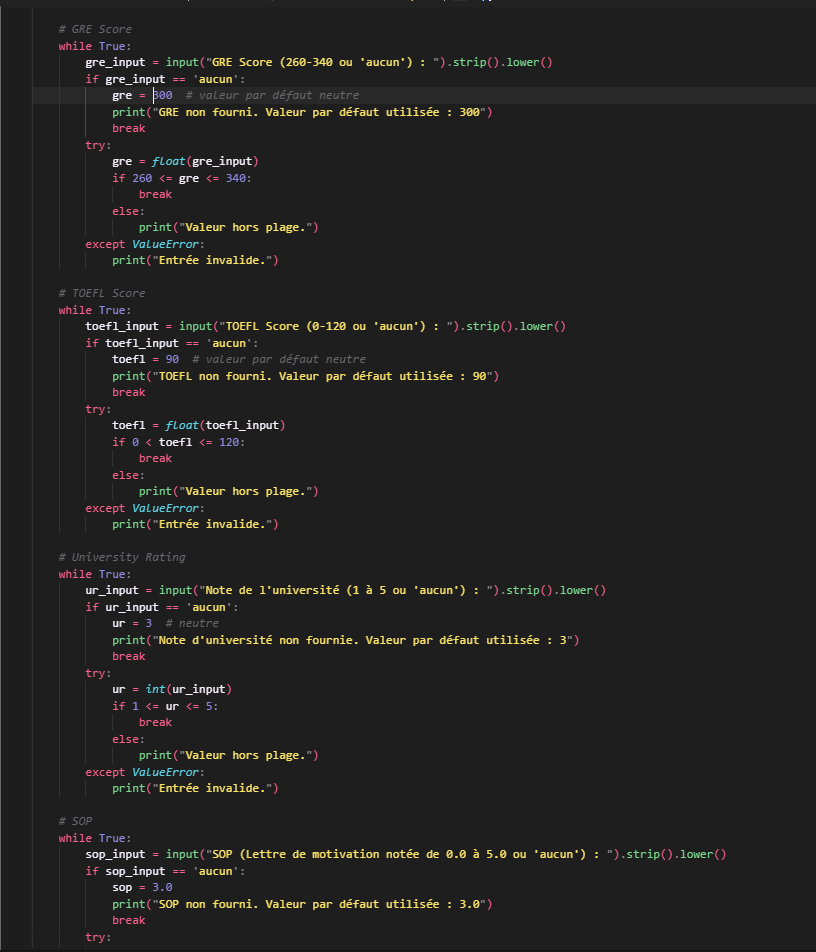
\includegraphics[width=0.9\textwidth]{../figures/t2.png}
	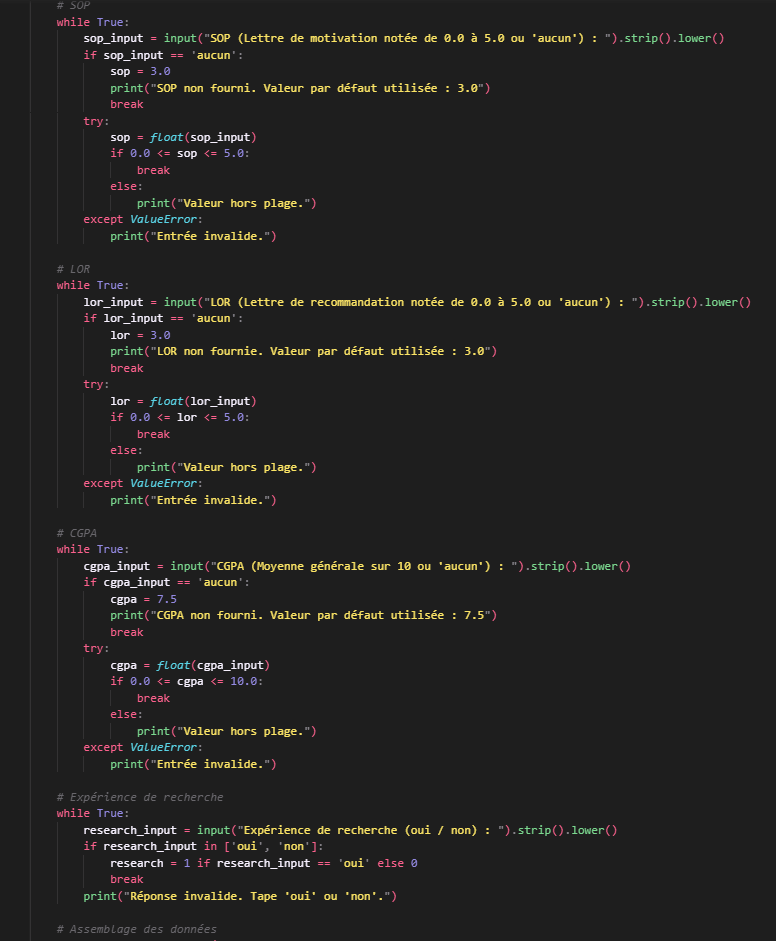
\includegraphics[width=0.9\textwidth]{../figures/t3.png}
	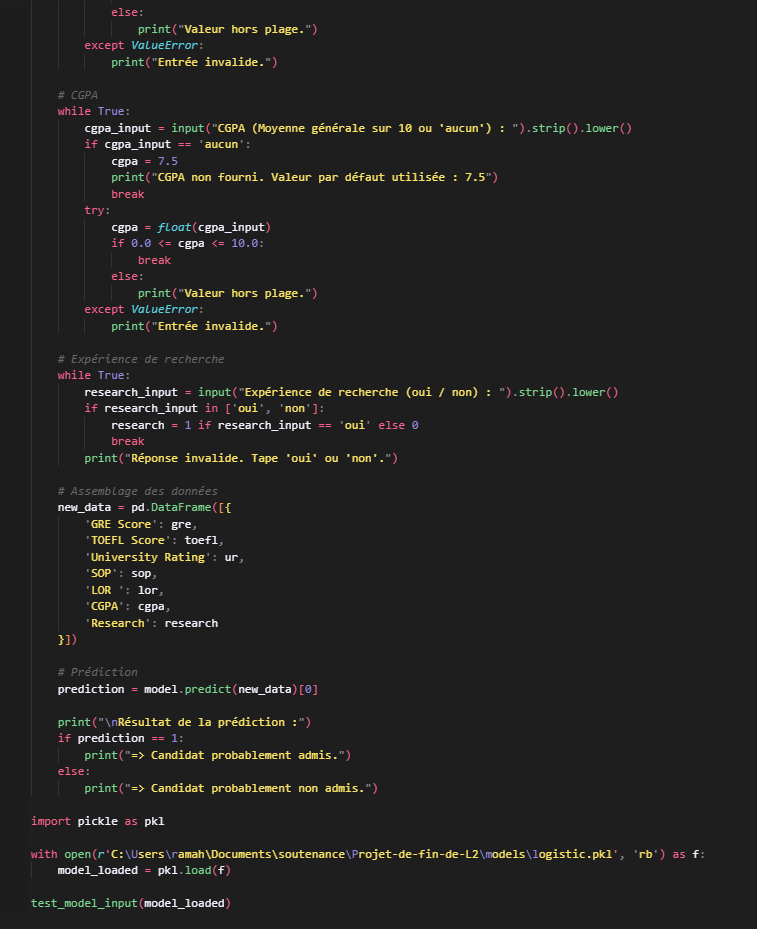
\includegraphics[width=0.9\textwidth]{../figures/t4.png}
\end{figure}
\noindent \textbf{Explication :} 
Ces extraits montrent l’évaluation du modèle sur le dataset de test, incluant la prédiction et l’analyse des performances.
